\documentclass[10pt,a4paper]{article}
\usepackage{CJKutf8}
\renewcommand{\tablename}{表}
\usepackage{geometry}
\usepackage{graphicx}
\usepackage{float}
\usepackage{multicol}
\usepackage{tcolorbox}
\tcbuselibrary{skins,breakable,raster}
\usepackage{array}
\tcbset{fonttitle=\bfseries,breakable,
	colback=white,
	every box/.style={enhanced,
		before=\par\smallskip,after=\par\smallskip},
	every box on layer 2/.style={reset,every box,colback=yellow!10!white,
		drop fuzzy shadow}}

\geometry{left=1cm,right=1cm,top=1cm,bottom=1.5cm}
\graphicspath{{img/}}
%\def\img#1#2{\begin{figure}[htb]\centering\includegraphics[width=0.7\columnwidth]{img/#1.png}\caption{#2}\label{fig:#1}\end{figure}}
\def\img#1#2{\begin{tcolorbox}[title=#2]\includegraphics[width=\textwidth]{#1.png}\end{tcolorbox}}
\def\pdf#1#2{\begin{tcolorbox}[title=#2]\includegraphics[width=\textwidth]{#1.pdf}\end{tcolorbox}}
\usepackage{enumitem}
\setlist{nosep}
\begin{document}
	\begin{CJK}{UTF8}{gbsn}
	\title{计算机组成}
	\date{}
	\begin{multicols}{3}
		\maketitle
		\section{微机}
		\textbf{微机结构}
\begin{itemize}
	\item Input 输入
	\item Output 输出
	\item Memory 存储器
	\item ALU 算术逻辑单元
	\item Control unit 控制单元
\end{itemize}

\begin{table*}
	\centering
	\caption{微机概念差异}
\begin{tabular}{|>{\bfseries}l|p{8cm}|}
	\hline
	微处理器 Microprocessor & 可以被微缩成集成电路规模的CPU电路,包含ALU,CU,寄存器 \\
	\hline
	微型计算机 Mircrocomputer & 微处理器,存储器,I/O,总线 \\
	\hline
	微型计算机系统 Microcomputer system & 以微型计算机为主体,配上I/O及系统软件就构成了微型计算机系统。 \\
	\hline
	微控制器 Microcontrollers & A microcontroller has a CPU in addition to a fixed amount of RAM, ROM, I/O ports on one single chip (\emph{e.g.} Cortex) \\
	\hline
	嵌入式系统 Embedded Systems & An embedded system uses a microcontroller or a microprocessor to do one task and one task only\\
	\hline
\end{tabular}
\end{table*}

\textbf{指令集}:CISC(1-n个字),RISC(1个字)

\textbf{字}:CPU一次可以处理的最大比特数

\textbf{位扩展}:同一地址的位扩展,满足一个字的输出

\textbf{字扩展}:增大字的量,选择不同的字,满足存储量需求

\begin{table*}
	\begin{minipage}{0.3\textwidth}
		\centering
		\caption{总线类型}
		\begin{tabular}{|c|c|c|}
			\hline
			\bfseries 类型 &\bfseries 仲裁 &\bfseries 时序 \\
			\hline
			单工 & 集中式 & 同步 \\
			多工 & 分布式 & 异步 \\
			\hline
		\end{tabular}
	\end{minipage}
	\begin{minipage}{0.7\textwidth}
		\centering
		\caption{总线结构}
		\begin{tabular}{|>{\bfseries}c|l|l|}
			\hline
			& \bfseries 优点 &\bfseries 缺点 \\
			\hline
			单线结构 & 简单 & 吞吐量低 \\
			\hline
			CPU-Central 双线结构 & 数据传输率高 & I/O与内存需要经过CPU \\
			\hline
			Memory-Central 双线结构 & CPU性能好 吞吐量高 &  \\
			\hline
		\end{tabular}
	\end{minipage}
\end{table*}


		\section{存储与I/O}
		\textbf{内存特征}
\begin{description}
	\item[Location]CPU,内部,外部
	\item[Capacity]字大小,字数目
	\item[Unit of transfer]内部(一字),外部(多字) --- Addressable Unit: 内部(一字节),外部(簇)
	\item[Access method] 访存方式
		\begin{itemize}
			\item Sequential 串行访问 (tape)
			\item Direct 直接访问 (disk)
			\item Random 随机访问 (RAM,ROM)
			\item Associative 关联访问 (cache)
		\end{itemize}
	\item[Performance] 评价指标
		\begin{itemize}
			\item Access time
			\item Memory Cycle time
			\item Transfer Rate
		\end{itemize}
	\item[Physical type] 物理类型
		\begin{itemize}
			\item Semiconductor (RAM)
			\item Magnetic (disk \& tape)
			\item Optical (CD \& DVD)
			\item Others (Bubble Hologram)
		\end{itemize}
	\item[Organisation] Physical arrangement of bits into words(存储字)
\end{description}

\begin{table*}
	\begin{minipage}[b]{.5\linewidth}
	\centering
	\caption{RAM 区别}
	\begin{tabular}{|>{\bfseries}l|c|c|}
		\hline
		& \bfseries DRAM &\bfseries SRAM \\
		\hline
		字节存储方式 & 电容电荷 & 开关状态 \\
		电荷泄漏 & 有 & 无 \\
		刷新 & 需要 & 不需要 \\
		构造 & 简单 & 复杂 \\
		每位规模 & 更小 & 更大 \\
		价格 & 便宜 & 昂贵 \\
		刷新电路 & 需要 & 不需要 \\
		速度 & 更慢 & 更快 \\
		用途 & 主存储器 & 高速缓存 \\
		\hline
	\end{tabular}
	\end{minipage}
	\begin{minipage}[b]{.5\linewidth}
	\centering
	\caption{ROM 区别}
	\begin{tabular}{|>{\bfseries}p{10em}|p{8em}|}
		\hline
		掩膜型 ROM & 无法修改 \\
		\hline
		可编程只读存储器 PROM & 一旦写入,不可改变 \\
		\hline
		可擦除可编程只读存储器 EPROM & 可写,用紫外光擦除,重新写入 \\
		\hline
		点可擦除的可编程只读存储器 EEPROM & 通电擦除,重新写入 \\
		\hline
		闪存 Flash & 对芯片编程,通电擦除再写入 \\
		\hline
	\end{tabular}
	\end{minipage}
\end{table*}

\textbf{I/O数据传送方式}
\begin{description}
	\item[程序控制方式 Programmed I/O] CPU与外设之间的数据传送是在程序控制下完成的。用查询方式使 CPU 与外设交换数据时,CPU要不断读取状态位,检查输入设备是否已准备好数据。由于许多外设的速度很低,这种等待过程会占去CPU的绝大部分时间,而真正用于传输数据的时间却很少,使CPU的利用率变得很低。
	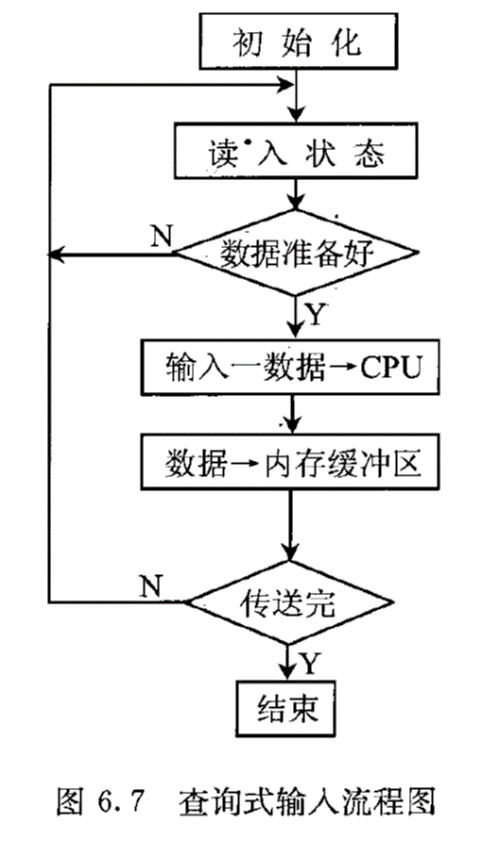
\includegraphics[width=0.75\columnwidth]{pinput.png}
	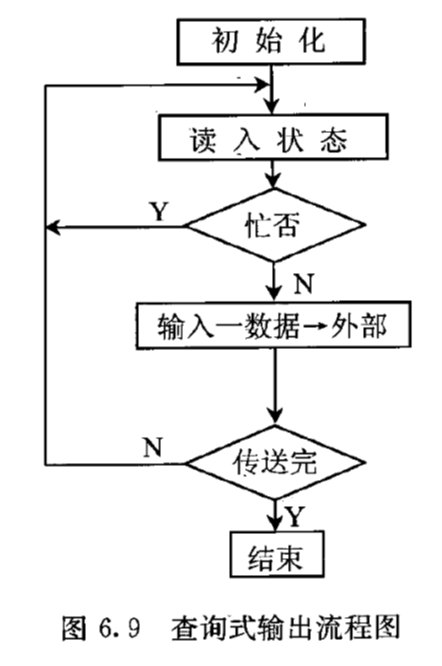
\includegraphics[width=0.75\columnwidth]{poutput.png}
	\item[中断方式 Interrupt driven I/O]采用中断方式后,CPU平时可以执行主程序,只有当输入设备将数据准备好了,或者输出端口的数据缓冲器已空时,才向CPU发中断请求。CPU响应中断后,暂停执行当前的程序,转去执行管理外设的中断服务程序(ISR)。在中断服务程序中,用于输入或输出指令在CPU和外设之间进行一次数据交换。等输入或输出操作完成之后,CPU又回去执行原来的程序。
	\begin{figure}[H]
	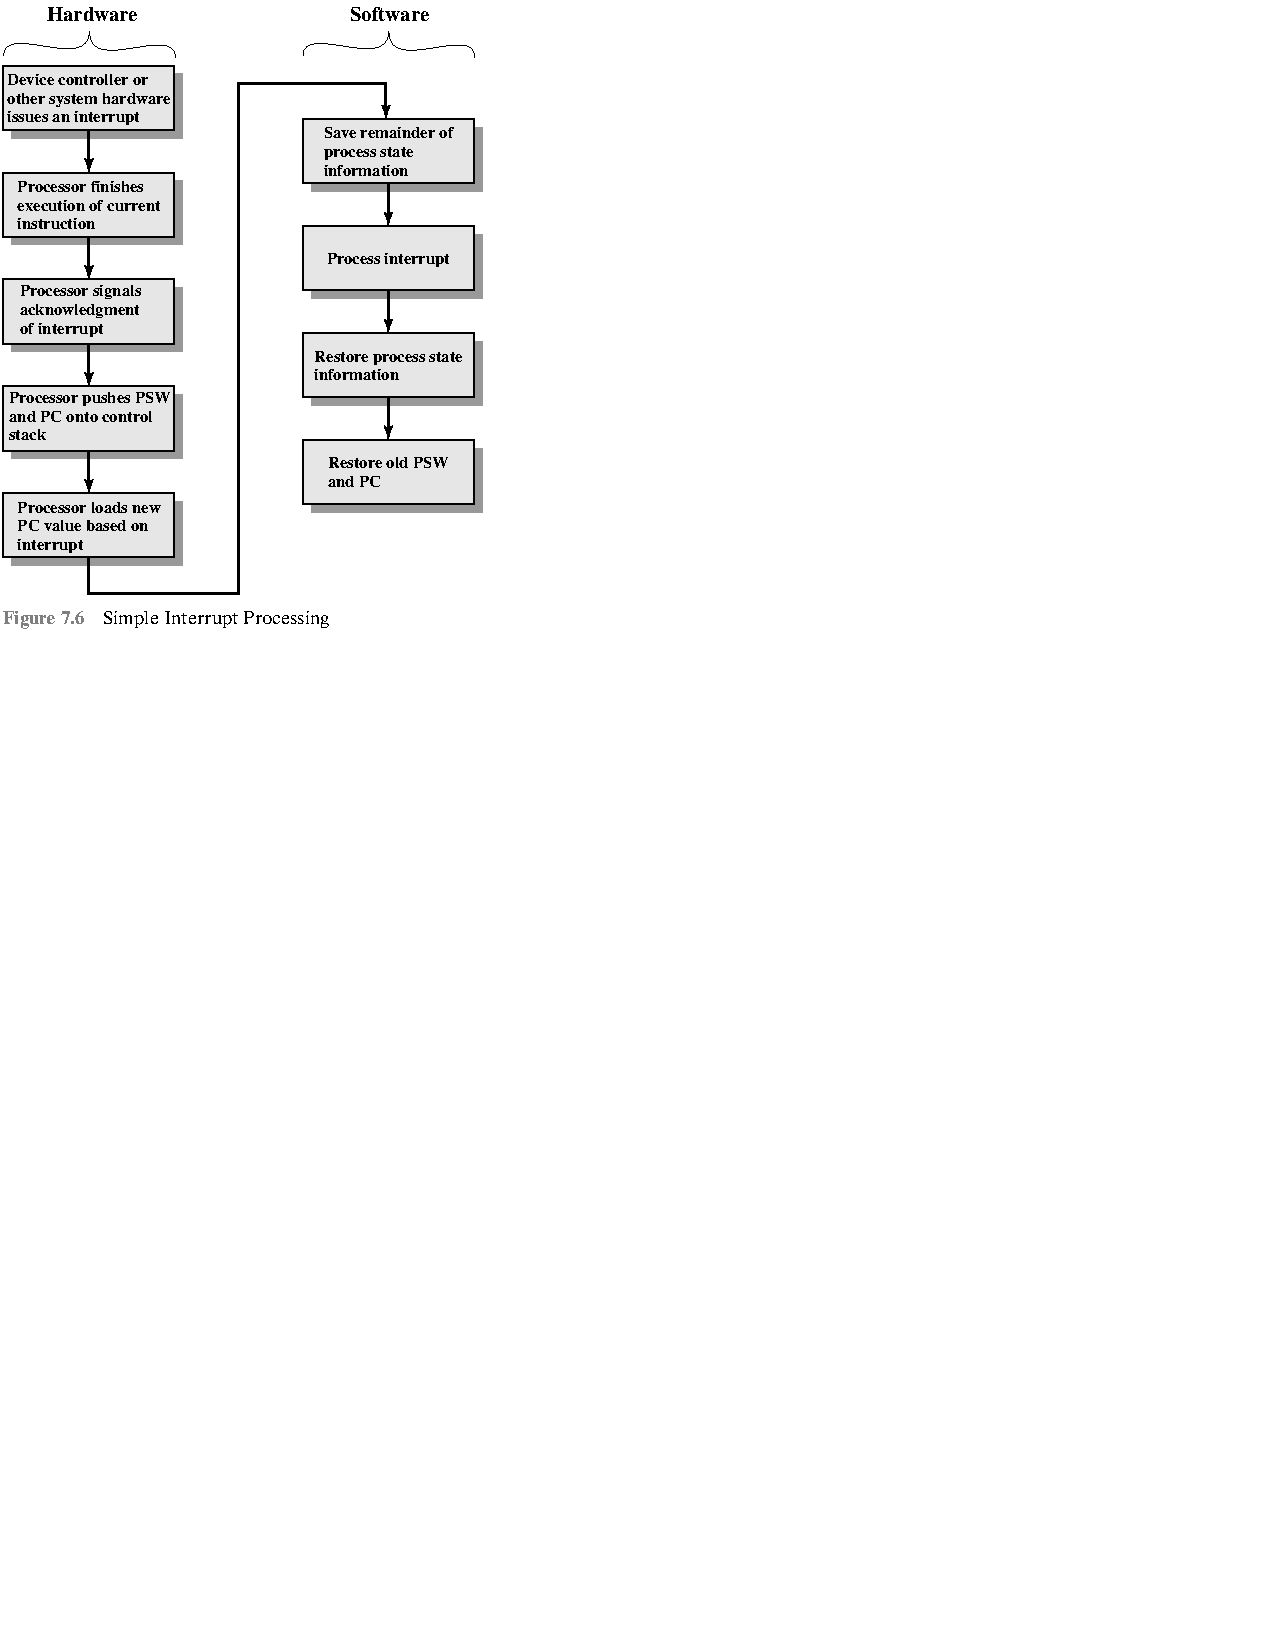
\includegraphics[width=\columnwidth]{interio.pdf}
	\end{figure}
	\item[直接存储器访问 DMA] DMA控制器临时接管总线,控制外设和存储器之间进行高速的数据传送,快速完成交换一批数据的任务,而不要CPU进行干预。这种控制器能给访问内存所需要的地址信息,并且能够自动修改地址指针,也能够设定和修改传送的字节数,还能够向存储器和外设发出相应的读写控制信号。在DMA传送结束后,它能够释放总线,把对总线的控制权又交还给CPU。
	\begin{figure}[H]
	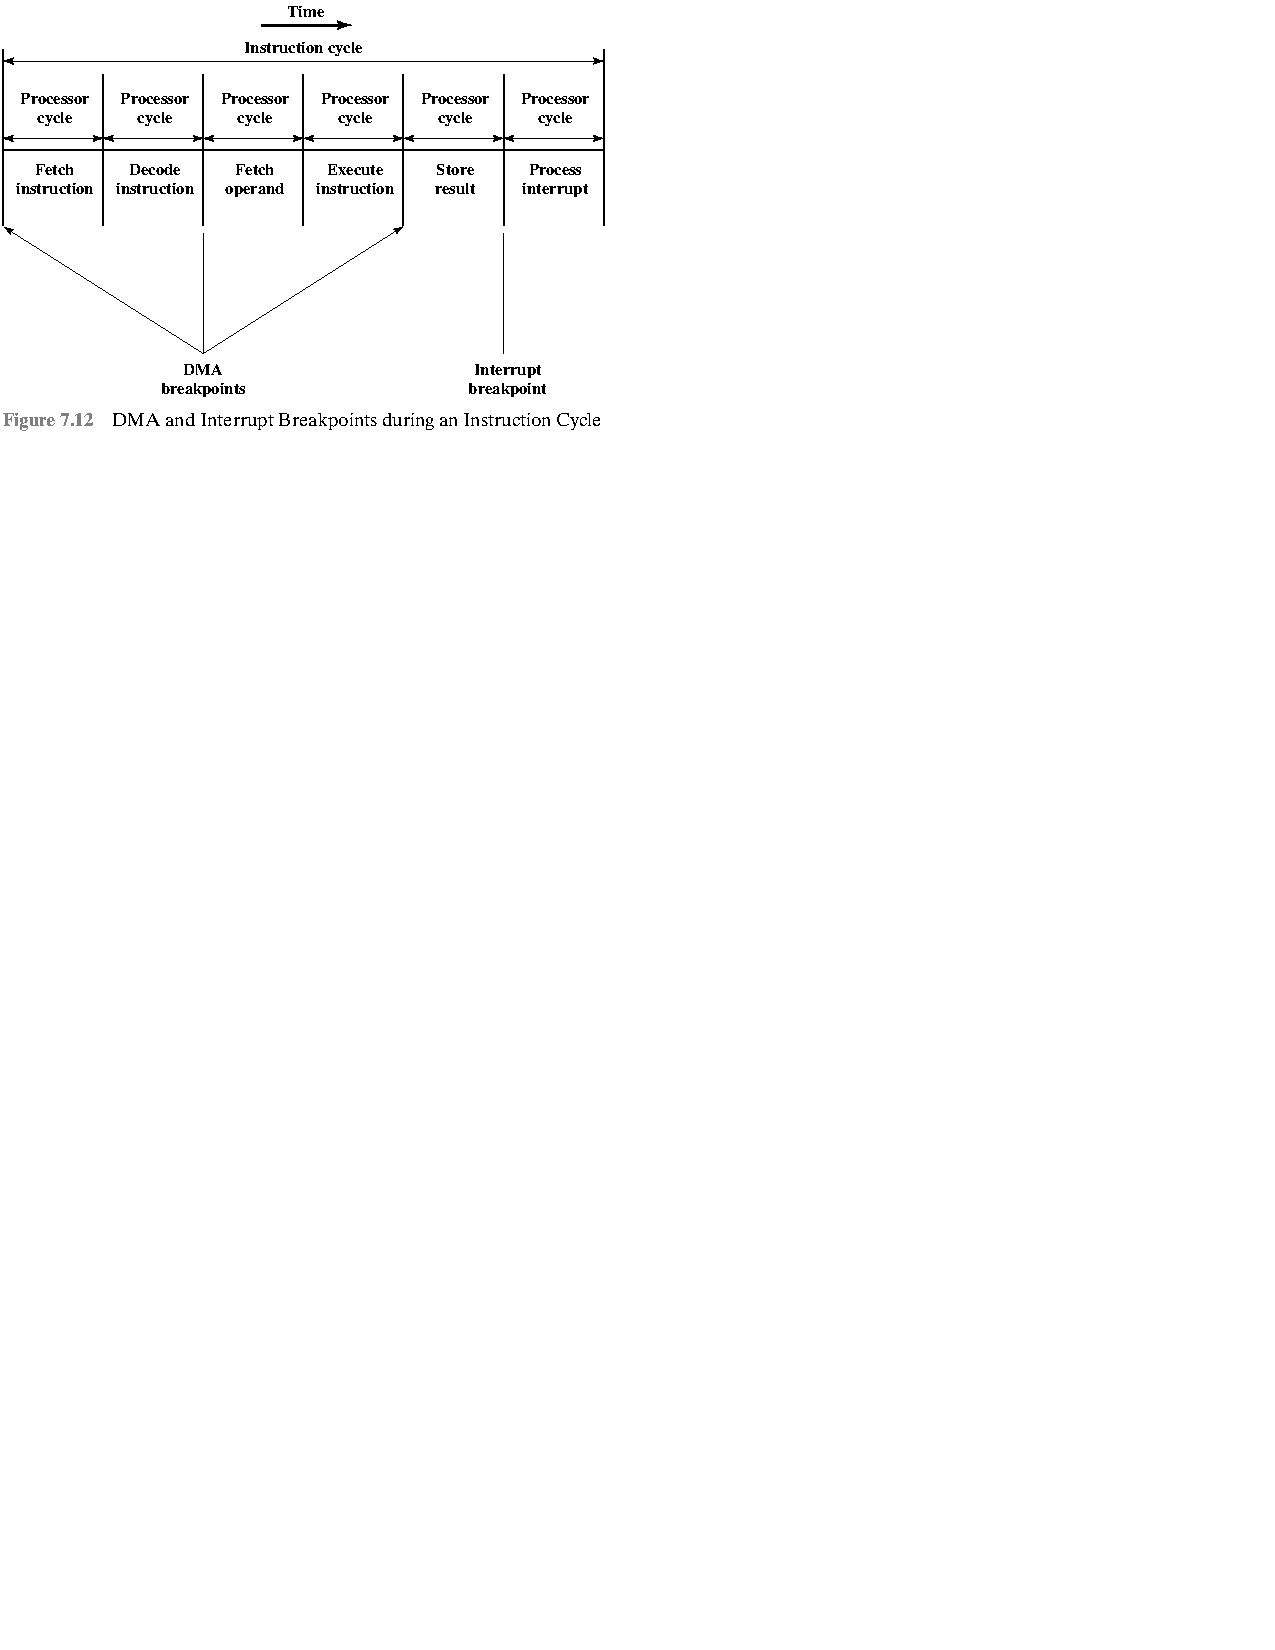
\includegraphics[width=\columnwidth]{DMA.pdf}
	\end{figure}
\end{description}

\begin{table*}
	\centering
	\caption{DMA 架构}
	\begin{tabular}{|>{\bfseries}l|c|c|}
		\hline
		& \bfseries 使用总线次数 &\bfseries CPU暂停次数 \\
		\hline
		Single Bus, Detached & 2 & 2 \\
		Single Bus,Intergrated & 1 & 1 \\
		Seperate I/O & 1 & 1 \\
		\hline
	\end{tabular}
\end{table*}

		\section{80x86}
		%\documentclass[10pt,a4paper]{article}
\usepackage{CJKutf8}
\renewcommand{\tablename}{表}
\usepackage{geometry}
\usepackage{graphicx}
\usepackage{float}
\usepackage{multicol}
%\usepackage{tcolorbox}
%\tcbuselibrary{skins,breakable,raster}
\usepackage{array}
%\tcbset{fonttitle=\bfseries,breakable,
%	colback=white,
%	every box/.style={enhanced,
%		before=\par\smallskip,after=\par\smallskip},
%	every box on layer 2/.style={reset,every box,colback=yellow!10!white,
%		drop fuzzy shadow}}

\geometry{left=1cm,right=1cm,top=1cm,bottom=1.5cm}
%\graphicspath{{img/}}
%\def\img#1#2{\begin{figure}[htb]\centering\includegraphics[width=0.7\columnwidth]{img/#1.png}\caption{#2}\label{fig:#1}\end{figure}}
\def\img#1#2{\begin{tcolorbox}[title=#2]\includegraphics[width=\textwidth]{#1.png}\end{tcolorbox}}
\def\pdf#1#2{\begin{tcolorbox}[title=#2]\includegraphics[width=\textwidth]{#1.pdf}\end{tcolorbox}}
\usepackage{enumitem}
\setlist{nosep}
\begin{document}
	\begin{CJK}{UTF8}{gbsn}
	\title{计算机组成}
	\date{}
%	\begin{multicols}{3}
\begin{description}
\item[8086] 16-bit, 20-bit address.
\item[8088] 16-bit internal, 8-bit external.
\end{description}

只有两段:
\begin{description}
	\item[BIU](Bus Interface Unit) 连接内存与外设。
	\item[EU](Execution Unit) 执行之前获取的指令。
\end{description}

\begin{table*}
	\centering
	\caption{8086 寄存器}
	\begin{tabular}{|>{\bfseries}l|c|l|}
		\hline
		Category & \bfseries Bits &\bfseries Register Names \\
		\hline
		General & 16 & \texttt{AX}(Accumulator), \texttt{BX}(Base), \texttt{CX}(Count), \texttt{DX}(Data) \\
		\hline
		& 8 & \texttt{AH}, \texttt{AL}, \texttt{BH}, \texttt{BL}, \texttt{CH}, \texttt{CL}, \texttt{DH}, \texttt{DL} \\
		\hline
		Pointer & 16 & \texttt{SP}(Stack Pointer), \texttt{BP}(Base Pointer) \\
		\hline
		Segment & 16 & \texttt{CS}(Code Segment), \texttt{DS}(Data Segment), \texttt{SS}(Stack Segment), \texttt{ES}(Extra Segment) \\
		\hline
		Instruction & 16 & \texttt{IP}(Instruction Pointer) \\
		\hline
		Flag & 16 & \texttt{FR}(Flag Register) \\
		\hline
	\end{tabular}
	\caption{段偏移寄存器}
	\begin{tabular}{|>{\bfseries}c|>{\ttfamily}c|>{\ttfamily}c|>{\ttfamily}c|>{\ttfamily}c|}
		\hline
		Segment register & CS & DS & ES & SS \\
		\hline
		Offset register & IP & SI,DI,BX & SI,DI,BX & SP,BP \\
		\hline
	\end{tabular}
	
\end{table*}

双工作模式
\begin{description}
	\item[最小模式] $\rm MN/\overline{MX}=1$ 单 CPU。
	\item[最大模式] $\rm MN/\overline{MX}=0$ 多 CPU(8086+8087),8288控制芯片。 
\end{description}

\begin{table*}
	\centering
	\caption{8086 接脚}
	\begin{tabular}{|>{\ttfamily}c|p{13em}|c|c|}
		\hline
		\bfseries Signal &\bfseries Description &\ttfamily 0 &\ttfamily 1 \\
		\hline
		ALE & Address Latch Enabled &  & Latched  \\
		\hline
		$\tt \overline{BHE}$ & Bank High Enabled & $\rm AD_8\sim \rm AD_{15}$ Enabled & $\rm AD_8\sim\rm AD_{15}$ Disabled \\
		\hline
		$\tt DT/\overline{R}$ & direction of Data Transfer & sending data & receiving data \\
		\hline
		$\tt \overline{DEN}$ & Data transceiver ENabled & enabled & disabled \\
		\hline
		$\tt \overline{WR}$ & WRiting to Mem/IO & writing & \\
		\hline
		$\tt \overline{RD}$ & ReaDing from mem/IO & reading & \\
		\hline
		$\tt M/\overline{IO}$ & CPU accessing Memory / IO & IO & Memory \\
		\hline
		$\tt INTR$ & INTerrupt Request, maskable by clearing IF &  & Requesting \\
		\hline
		$\tt \overline{INTA}$ & INTerrupt Acknowledge &  & Acknowledge \\
		\hline
		$\tt NMI$ & Non-Maskable Interrupt, CPU is interrupted after finishing the current instruction; cannot be masked by software &  & will be interrupted \\
		\hline
		$\tt HOLD$ & HOLD the bus request &  & hold \\
		\hline
		HLDA & HoLD request acknowledge &  & hold req ack \\
		\hline
		$\tt \overline{TEST}$ & for debug & test &  \\
		\hline
		READY & mem/IO is READY for transfer &  & ready \\
		\hline
		RESET & reset the CPU, IP, DS, SS, ES and 6 inst in instruction queue are cleared &  & CS=\texttt{0FFFFH} \\
		\hline
	\end{tabular}
\end{table*}

%\begin{figure}[H]
%	\centering
%	\caption{8086/88 周期}
%	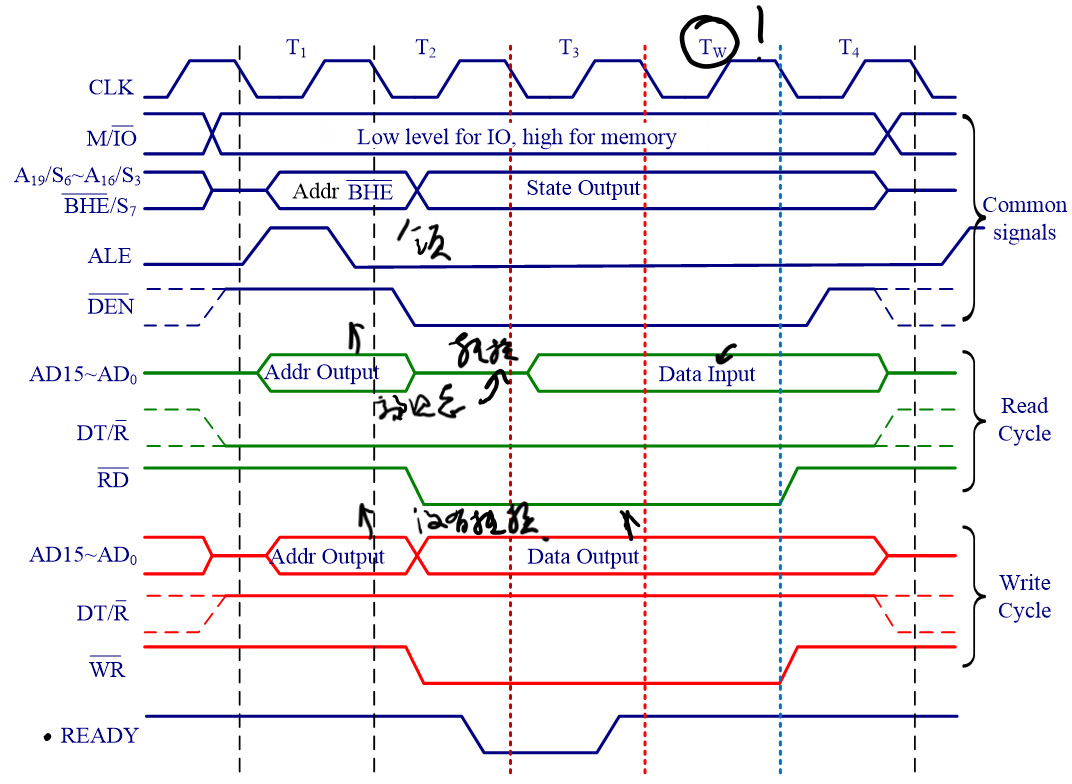
\includegraphics[width=\textwidth]{buscycle.png}
%\end{figure}
8086读周期时序:
在8086读周期内,有关总线信号的变化如下:
\begin{enumerate}
\item M/IO在整个读周期保持有效,当进行存储器读操作时,M/IO为高电平;当进行I/O端口读操作时,M/IO为低电平.
\item A19/S6~A16/S3是在T1期间,输出CPU要读取的存储单元的地址高4位.T2~T4期间输出状态信息S6~S3.
\item BHE/S7在T1期间输出BHE有效信号(BHE为低电平),表示高8位数据总线上的信息可以使用,BHE信号通常作为奇地址存储体的选择信号(偶地址存储体的选择信号是最低地址位A0).T2~T4期间输出高电平.
\item ADl5~AD0在T1期间输出CPU要读取的存储单元或I/O端口的地址A15~A0.T2期间为高阻态,T3~T4期间,存储单元或I/O端口将数据送上数据总线.CPU从ADl5~AD0上接收数据.
\item ALE:在T1期间地址锁存有效信号,为一正脉冲,系统中的地址锁存器正是利用该脉冲的下降沿来锁存A19/S6~A16/S3,ADl5~AD0中的20位地址信息以及BHE.
\item RD在T2期间输出低电平,送到被选中的存储器或I/O接口.要注意的是,只有被地址信号选中的存储单元或I/O端口,才会被RD信号从中读出数据(数据送上数据总线ADl5~AD0).
\item DT/R在整个总线周期内保持低电平,表示本总线周期为读周期.在接有数据总线收发器的系统中,用来控制数据传输的方向.
\item DEN在T2~T3期间输出有效低电平,表示数据有效.在接有数据总线收发器的系统中,用来实现数据的选通.
\end{enumerate}

8086写周期时序总线写操作的时序与读操作时序相似,其不同处在于:
\begin{enumerate}
\item 	
AD15~AD0在T2~T4期间送上欲输出的数据,而无高阻态.
\item WR在T2~T4期间输出有效低电平,该信号送到所有的存储器和I/O接口.要注意的是,只有被地址信号选中的存储单元或I/O端口才会被WR信号写入数据.
\item DT/R在整个总线周期内保持高电平,表示本总线周期为写周期.在接有数据总线收发器的系统中,用来控制数据传输方向.
\end{enumerate}

%%\end{multicols}
\end{CJK}
\end{document}
	\end{multicols}
	\begin{twocolumn}
%		\begin{multicols}{3}
%		\begin{tcbraster}[raster columns=3, raster equal height,
%			]
		\img{von}{冯诺依曼结构}
		\img{harvard}{哈佛结构}
		\img{struct}{微机结构}
		\img{sysstruct}{微机系统结构(哈佛结构)}
		\img{memhier}{内存层级}
		\img{memorg}{内存组织}
		\begin{tcolorbox}[title=总线结构]
		\img{singlebus}{单线结构}
		\img{dualbus}{CPU-Central 双线结构}
		\img{memdualbus}{Memory-Central 双线结构}
		\end{tcolorbox}
		\begin{tcolorbox}[title=寻址方式]
			\img{memio}{存储器映像寻址方式}
			\begin{tcolorbox}[title=I/O单独编址方式]
				\img{isoiod}{单工地址线}
				\img{isoiom}{多工地址线}
			\end{tcolorbox}
		\end{tcolorbox}
		\begin{tcolorbox}[title=RAM]
%			\begin{tcbraster}[raster columns=2,raster equal height=rows,]
%				\img{DRAM}{DRAM}
%				\img{SRAM}{SRAM}
%			\end{tcbraster}
			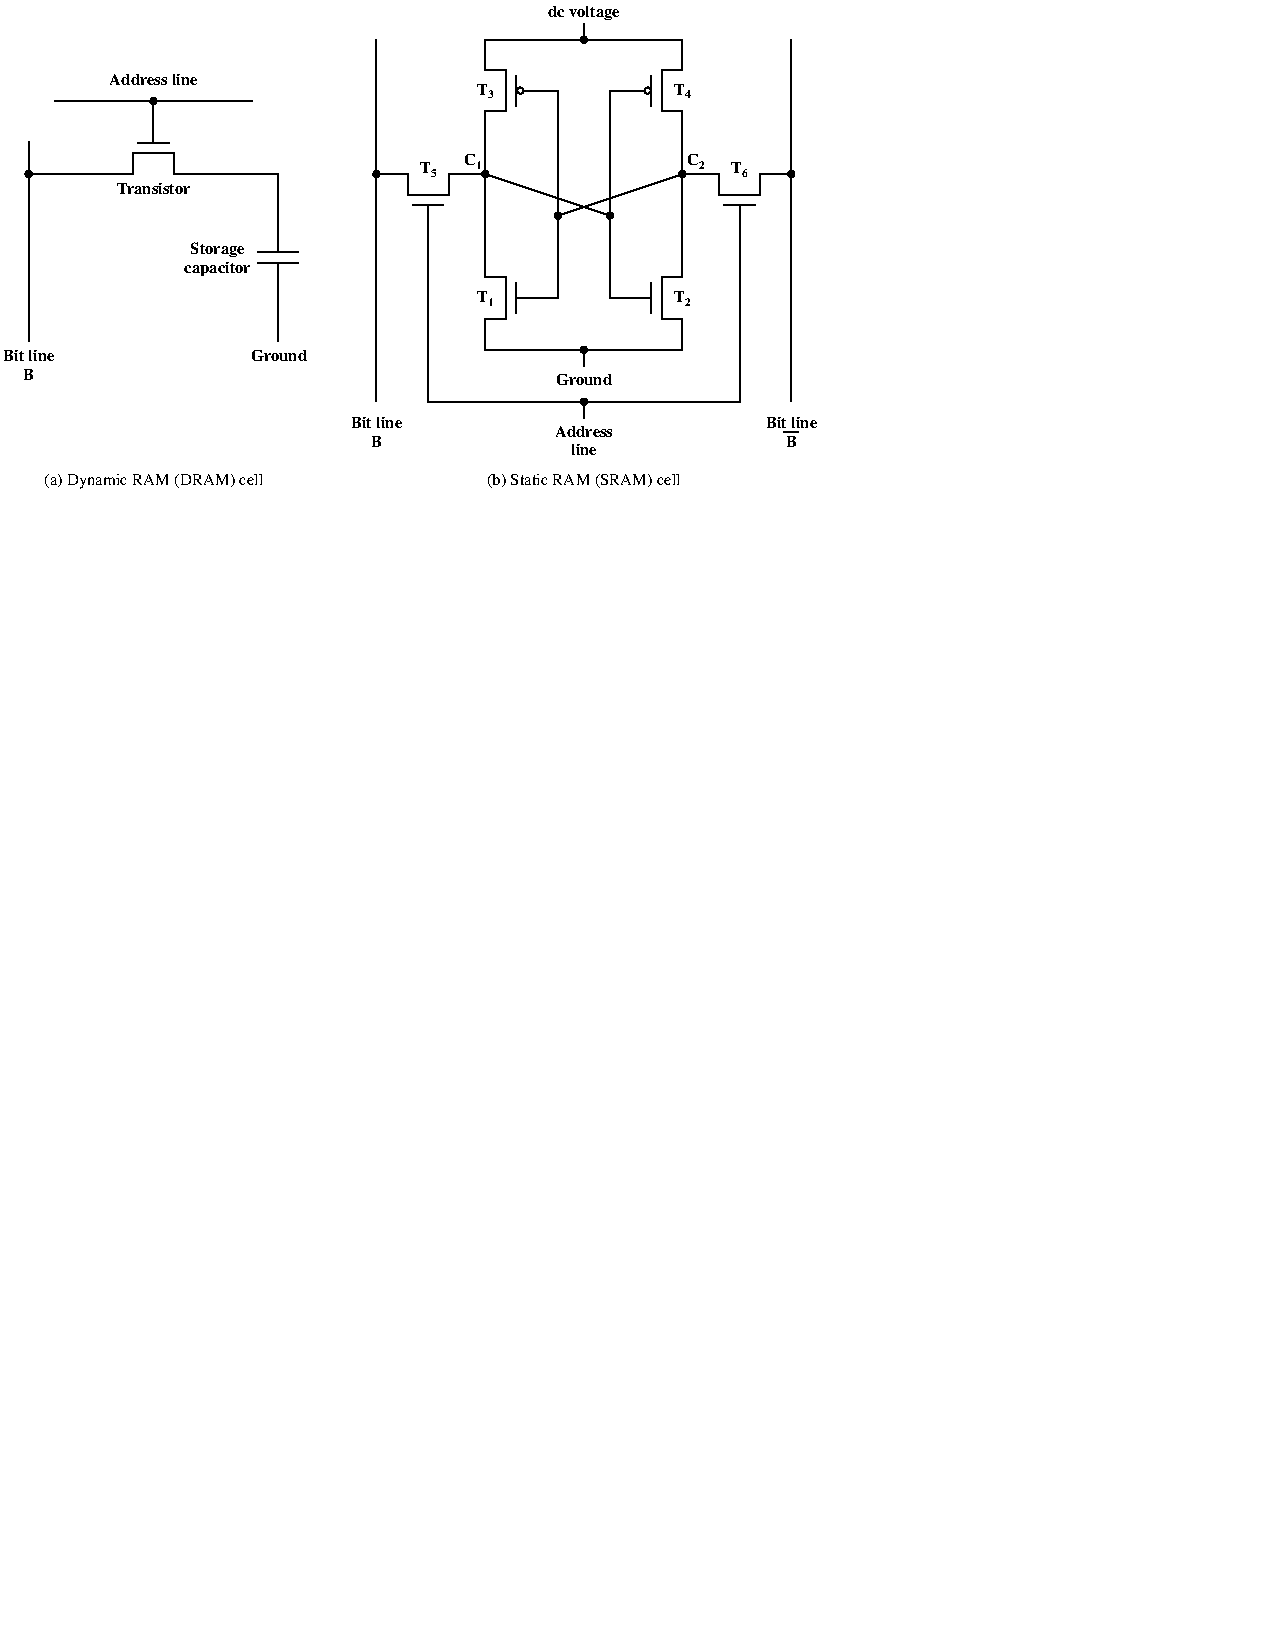
\includegraphics[width=\textwidth]{RAM.pdf}
		\end{tcolorbox}
		\pdf{DRAM16}{4M$\times$4 DRAM}
		\pdf{pkg}{存储芯片封装}
		\begin{tcolorbox}[title=存储位扩展]
			\pdf{bitext}{256K$\times$8-bit: 8 256$\times$1-bit}
			\img{bitext}{256K$\times$32-bit: 32 256K$\times$1-bit}
		\end{tcolorbox}
		\begin{tcolorbox}[title=存储字扩展]
			\pdf{wordext}{1M$\times$8-bit: 4 group 256K$\times$1-bit}
			\img{wordext}{2M$\times$8-bit: 8 group 256K$\times$8-bit}
		\end{tcolorbox}
		\begin{tcolorbox}[title=字与位同时扩展]
			\img{wbext}{32位可寻址单元}
			\img{wbextb}{1字节可寻址单元}
		\end{tcolorbox}
		\pdf{pref}{外设}
		\pdf{iomod}{I/O模块}
		\pdf{interrupt}{中断处理内存变化}
		\pdf{DMAalter}{DMA架构}
		\img{8086}{8086内部结构}
		\img{8086l}{8086配置图}
		\begin{tcolorbox}[title=逻辑门电路]
			\centering
			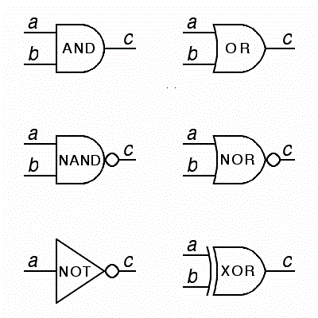
\includegraphics[width=0.75\textwidth]{CMOS.png}
%			\includegraphics[width=\textwidth]{logic.jpg}
			\begin{tabular}{|c|c|c|c|c|c|c|c|}
				\hline
				\multicolumn{2}{|c|}{input} & \multicolumn{6}{c|}{output} \\
				\hline
				$ a $ & $ b $  & $ ab $ & $ a+b $ & $ \overline{ab} $ & $ \overline{a+b} $& $\overline{a}$ & $a\oplus b$ \\
				\hline
				0 & 0 & 0 & 0 & 1 & 1 & 1 & 0 \\
				\hline
				0 & 1 & 0 & 1 & 1 & 0 & 1 & 1 \\
				\hline
				1 & 0 & 0 & 1 & 1 & 0 & 0 & 1 \\
				\hline
				1 & 1 & 1 & 1 & 0 & 0 & 0 & 0 \\
				\hline
			\end{tabular}
		\end{tcolorbox}
		\begin{tcolorbox}[title=锁存器和数据传输器]
			\img{latch}{74LS373 D Latch}
			\img{dt}{Data Bus Transceiver}
		\end{tcolorbox}
		\img{buscycle}{8086/88 总线周期}
%		\end{tcbraster}
%		\end{multicols}
	\end{twocolumn}
	\end{CJK}
\end{document}